\chapter{Computational methods}
\section{Introduction} % TODO Update from MRes version
Computational techniques are a vital tool in the prediction and characterisation of solid state materials.
Not only can computational methods reduce experimental load by identifying promising material candidates in screening studies, but they can offer atomic scale insights into the structural and transport properties of materials not observable by experiment.

This study primarily uses potentials-based minimisation techniques and Molecular Dynamics (MD), implemented in GULP \cite{Gale2003} and LAMMPS \cite{StevePlimton1995} respectively.
In this chapter, the fundamental concepts and mathematics underpinning these techniques are presented.
Furthermore, an overview of classical interatomic potential fitting strategies are presented and contrasted with in development techniques.to contrast to the work presented herein. %TODO chapter reference
This overview is brief and focuses primarily on techniques used in this report, as more comprehensive reviews are available elsewhere. \cite{Gale2003, Jensen2007, Catlow2013}
Some work presented in this section is derived from the MRes report which led to this project, as the fundamental equations underpinning computational methods remain the same.

\section{Atomistic modelling}
An understanding of the forces atoms experience as a function of their environment is vital to gain insights into the properties of systems of interest.
One class of approaches for calculating the interatomic forces between atoms, \textit{ab initio} techniques, are based on quantum mechanics, and seek to determine electron density as a function of position. Whilst the scale of systems these strategies can be used for is increasing with developments in computational resource available, these techniques remain prohibitively expensive for large systems or systems studied over large time-scales.

In contrast, atomistic techniques seek to express the forces between atoms as a series of empirically derived models, either fitted to experimental or \textit{ab initio} data, which can be cheaply evaluated, allowing for large scale systems to be studied over large time scales. This is particularly important when considering phenomenon which occur over large time scales, such as diffusion. 

\section{Potential models}
All atoms in a system, and their current position, momentum, and oxidation state, give rise to highly complex interactions contributing to the internal energy of the system, which must be enumerated if a perfect atomistic model is to be developed.

Potential models are used to determine the forces in such systems by treating these as a series of discrete isolated interactions which sum to the same overall effect. 
The internal energy of the system can then be given as the sum from one to n-body terms as such:\cite{Gale2003}
\begin{align}
U &=& &\sum_{i = 1} U_i&         &+& &\frac{1}{2}\sum_{i = 1} \sum_{j = 1} U_{ij}&  &+& &\frac{1}{6}\sum_{i = 1} \sum_{j = 1} \sum_{k = 1} U_{ijk}& &+& &\cdots\\
&=& &\sum_{i = 1}^\prime U_i&  &+& &\sum_{i,j = 1}^\prime U_{ij}&                 &+& &\sum_{i,j,k = 1}^\prime U_{ijk}&                           &+& &\cdots
\label{eq:taylor}
\end{align}
With the first term accounting for single-body terms, the second term accounting for those interactions which exist between pairs of bodies and so on.
The primed sum in Equation \ref{eq:taylor} distinguishes between interactions that are enumerated repeatedly, and instead counts each unique interaction only once, hence cancelling the $\frac{1}{N!}$ term.
This expansion is exact if expanded to account for all N-body interactions in a system.

As it is only the low order terms which give rise to the majority of the internal energy of a system, it suffices to truncate this expansion to lower order terms.
Typically, this is limited to two-body terms, although higher order terms are included where these strongly impact the system (e.g. bond angles).
Beyond this, higher order terms are only considered where the calculation of a specific property of interest requires their inclusion.
Three-body interactions are required to calculate phonon distribution curves for example.

Furthermore, as the number of bodies in an interaction increases, it becomes increasingly difficult to find a rational physical basis on which an empirical model can be based. 
 
Single body interactions are implemented to represent an external forcefield being applied to a system, such as the application of an external electric field interacting with charged species.
They are also used in the Einstein model, in which species do not interact with one another, and instead are attached to their lattice sites by a spring term.
Single body terms are not used in the course of this study, but are referenced here for completeness sake.
\subsection{Two-body interactions}
The two-body terms in Equation \ref{eq:taylor}: 
\begin{equation}
\sum_{i,j = 1}^\prime U_{ij}
\end{equation}
account for the interactions occurring between pairs of atoms or ions in isolation.
As no reference frame is given, these terms are therefore strictly a function of interatomic separation.
It is conventional to further subdivide these two-body interactions into Coulombic (long-range) and short-range terms as so:
\begin{equation}
U_{ij} = \Phi_{Coulombic} + \Phi_{short-range}
\label{eq:two-body}
\end{equation}

The Coulombic term in Equation \ref{eq:two-body} is the potential arising from electrostatic interactions between pairs of charged species:

\begin{equation}
\Phi_{Coulombic} = \frac{q_iq_j}{r_{ij}}
\label{eq:coulombic}
\end{equation}
Where $q_i$ and $q_j$ are the effective charges of the species.
This term is colloquially referred to as the ``long-range'' term, as the non-Coulombic component of these interactions are comparatively tiny beyond a certain range.
It is also typically the dominant component in a system at equilibrium, accounting for around 90\% of the total potential energy in a usual system.\cite{Catlow2013}

The long-range nature of the Coulombic term leads to slow convergence in direct space for a large number of ions.
The \citet{Ewald1921} summation can be used to overcome this shortcoming in periodic systems, by further subdividing the Coulombic interactions into short- and long-range terms.
The short-range components are computed as before, while the long-range terms are solved in reciprocal space.

The nature of a two-body interaction can vary widely dependent on context, with the species, charge, and even local environment impacting the resultant potential.
Depending on the system, covalent interactions, London interactions and electron-pair repulsions may all need to be accounted for with no actual calculation of electron density occurring on which to base the potential.

This can include electron-pair repulsions, London interactions and covalent interactions.
This term can be calculated through the use of tabulated data, or via simple analytical models.
Analytical models are typically empirically derived from experimental data.

The selection of an appropriate model is vital, with considerations including the ionic/covalent nature of the system, availability of experimental data, and computational cost influencing the choice of model.
Furthermore, given potential models are often derived to match experimental data for a given system, ensuring that that same potential is suitable when applied outside of the context in which it was developed is important.

This of course can pose an issue when seeking to study systems where no experimental data is available with which to verify the findings of computational work.
 For ionic systems, the Buckingham Potential form is conventionally used to for two-body interactions:


\begin{equation}
\Phi_{ij} = A\cdot \exp \left(\frac{-r_{ij}}{\rho_{ij}} \right) - \frac{C}{r_{ij}^6}
\label{eq:Buckingham}
\end{equation}

\noindent Other common short range potential models are given in Table \ref{tab:potentialmodels}

\begin{table}[t]
  \centering
  \caption{Common short-range two-body potential models.\cite{Gale2003}}
  \label{tab:potentialmodels}
  \begin{tabular}{@{}lc@{}}
  \toprule
  Potential Model         & Expression     \\
  \midrule
  Buckingham              & $\displaystyle{\Phi_{ij} = A\cdot \exp \left(\frac{-r_{ij}}{\rho_{ij}} \right) - \frac{C}{r_{ij}^6}}$    \\
  \addlinespace
  Harmonic                & $\displaystyle{\Phi_{ij} = \frac{1}{2}k_2(r_{ij}-r_0)^2   + \frac{1}{6}k_3(r_{ij}-r_0)^3    + \frac{1}{24}k_4(r_{ij}-r_0)^4   }$    \\
  \addlinespace
  Lennard-Jones           & $\displaystyle{\Phi_{ij} = \left(\frac{A}{r_{ij}^m} \right) - \left( \frac{B}{r_{ij}^n}\right)}$   \\
  \addlinespace
  Morse                   & $\displaystyle{\Phi_{ij} = D_e \left((1- \exp(-a(r_{ij} - r_0)))^2           -1\right) }$    \\
  \bottomrule
  \end{tabular}
\end{table}

\vspace{-5pt}
\paragraph{Finite-range implementation}
As the name suggests, the short-range terms dominate in the short-range, but the force arising from these interactions decreases rapidly with increasing interatomic distance.
To decrease the computational expense, a threshold radius is defined beyond which all forces are assumed to be zero.
The selection of this threshold is important, as the computational expense is of $O(r_t^2)$, so the shorter this radius the less expensive the simulation, whereas too small a radius will result in a change in the simulation result and decrease in model quality.

In order to prevent this strategy introducing discontinuity into the system, additional terms are added to smoothly reduce the interatomic potential and associated energy derivatives to zero at the threshold radius. %TODO rephrase


\subsection{Three-body interactions}
The nature of three-body terms are dependant on the interactions between three ions or atoms.
These can be interpreted as bond pair repulsions or as a charge dispersion between three bodies in covalent and ionic interpretations respectively.
This term is small relative to the two-body terms, and is usually only included when high degrees of accuracy are required, or for the calculation of properties dependent on three-body interactions such as phonon distribution curves.

A commonly used three-body potential is the harmonic model:
\begin{equation}
  U_{ijk} = \frac{1}{2}k_2(\theta-\theta_0)^2   + \frac{1}{6}k_3(\theta-\theta_0)^3    + \frac{1}{24}k_4(\theta-\theta_0)^4
  \label{eq:threebody}
\end{equation}

In this model, an equilibrium angle is assigned to a bond pair, and any deviations from this angle increase the potential energy of the system.

\subsection{Polarizability}
The electron distribution surrounding an atom or ion will shift according to the local environment in which it exists, effectively allowing the internuclear and electronic interactions to partially decouple.
A rigid ion model, in which species are modelled as point charges, does not capture this behaviour, defreasing the accuracy of models using it.
This is a particularly important behaviour when studying ion migration, and so a failure to account for this behaviour can negatively impact the accuracy of results obtained.

An early model of ion polarisation is the point polarisable ion model (PPI), in which the dipole moment of an ion ($\mu$) is directly proportional to the strength of the electric field in which it sits(E):
\begin{equation}
\mu = \alpha E
\end{equation}
Whilst computationally inexpensive and easily extensible to higher order polarizabilities (i.e. quadrupolar systems), this model performs poorly when handling dynamic lattice properties.
It also poorly predicts dielectric constants, which is easily measurable experimentally and thus a useful criteria for model validation.

This shortcoming can be rationalised by the failure to account for the polarisation of adjacent ions, that is, that neighbouring species being polarised impacts the local electric field and serves to dampen polarisation overall.
Consequently, this model tends to overestimate dielectric constants if tuned to accurately predict another physical property (e.g. elastic constants).


\begin{figure}[ht]
  \centering
  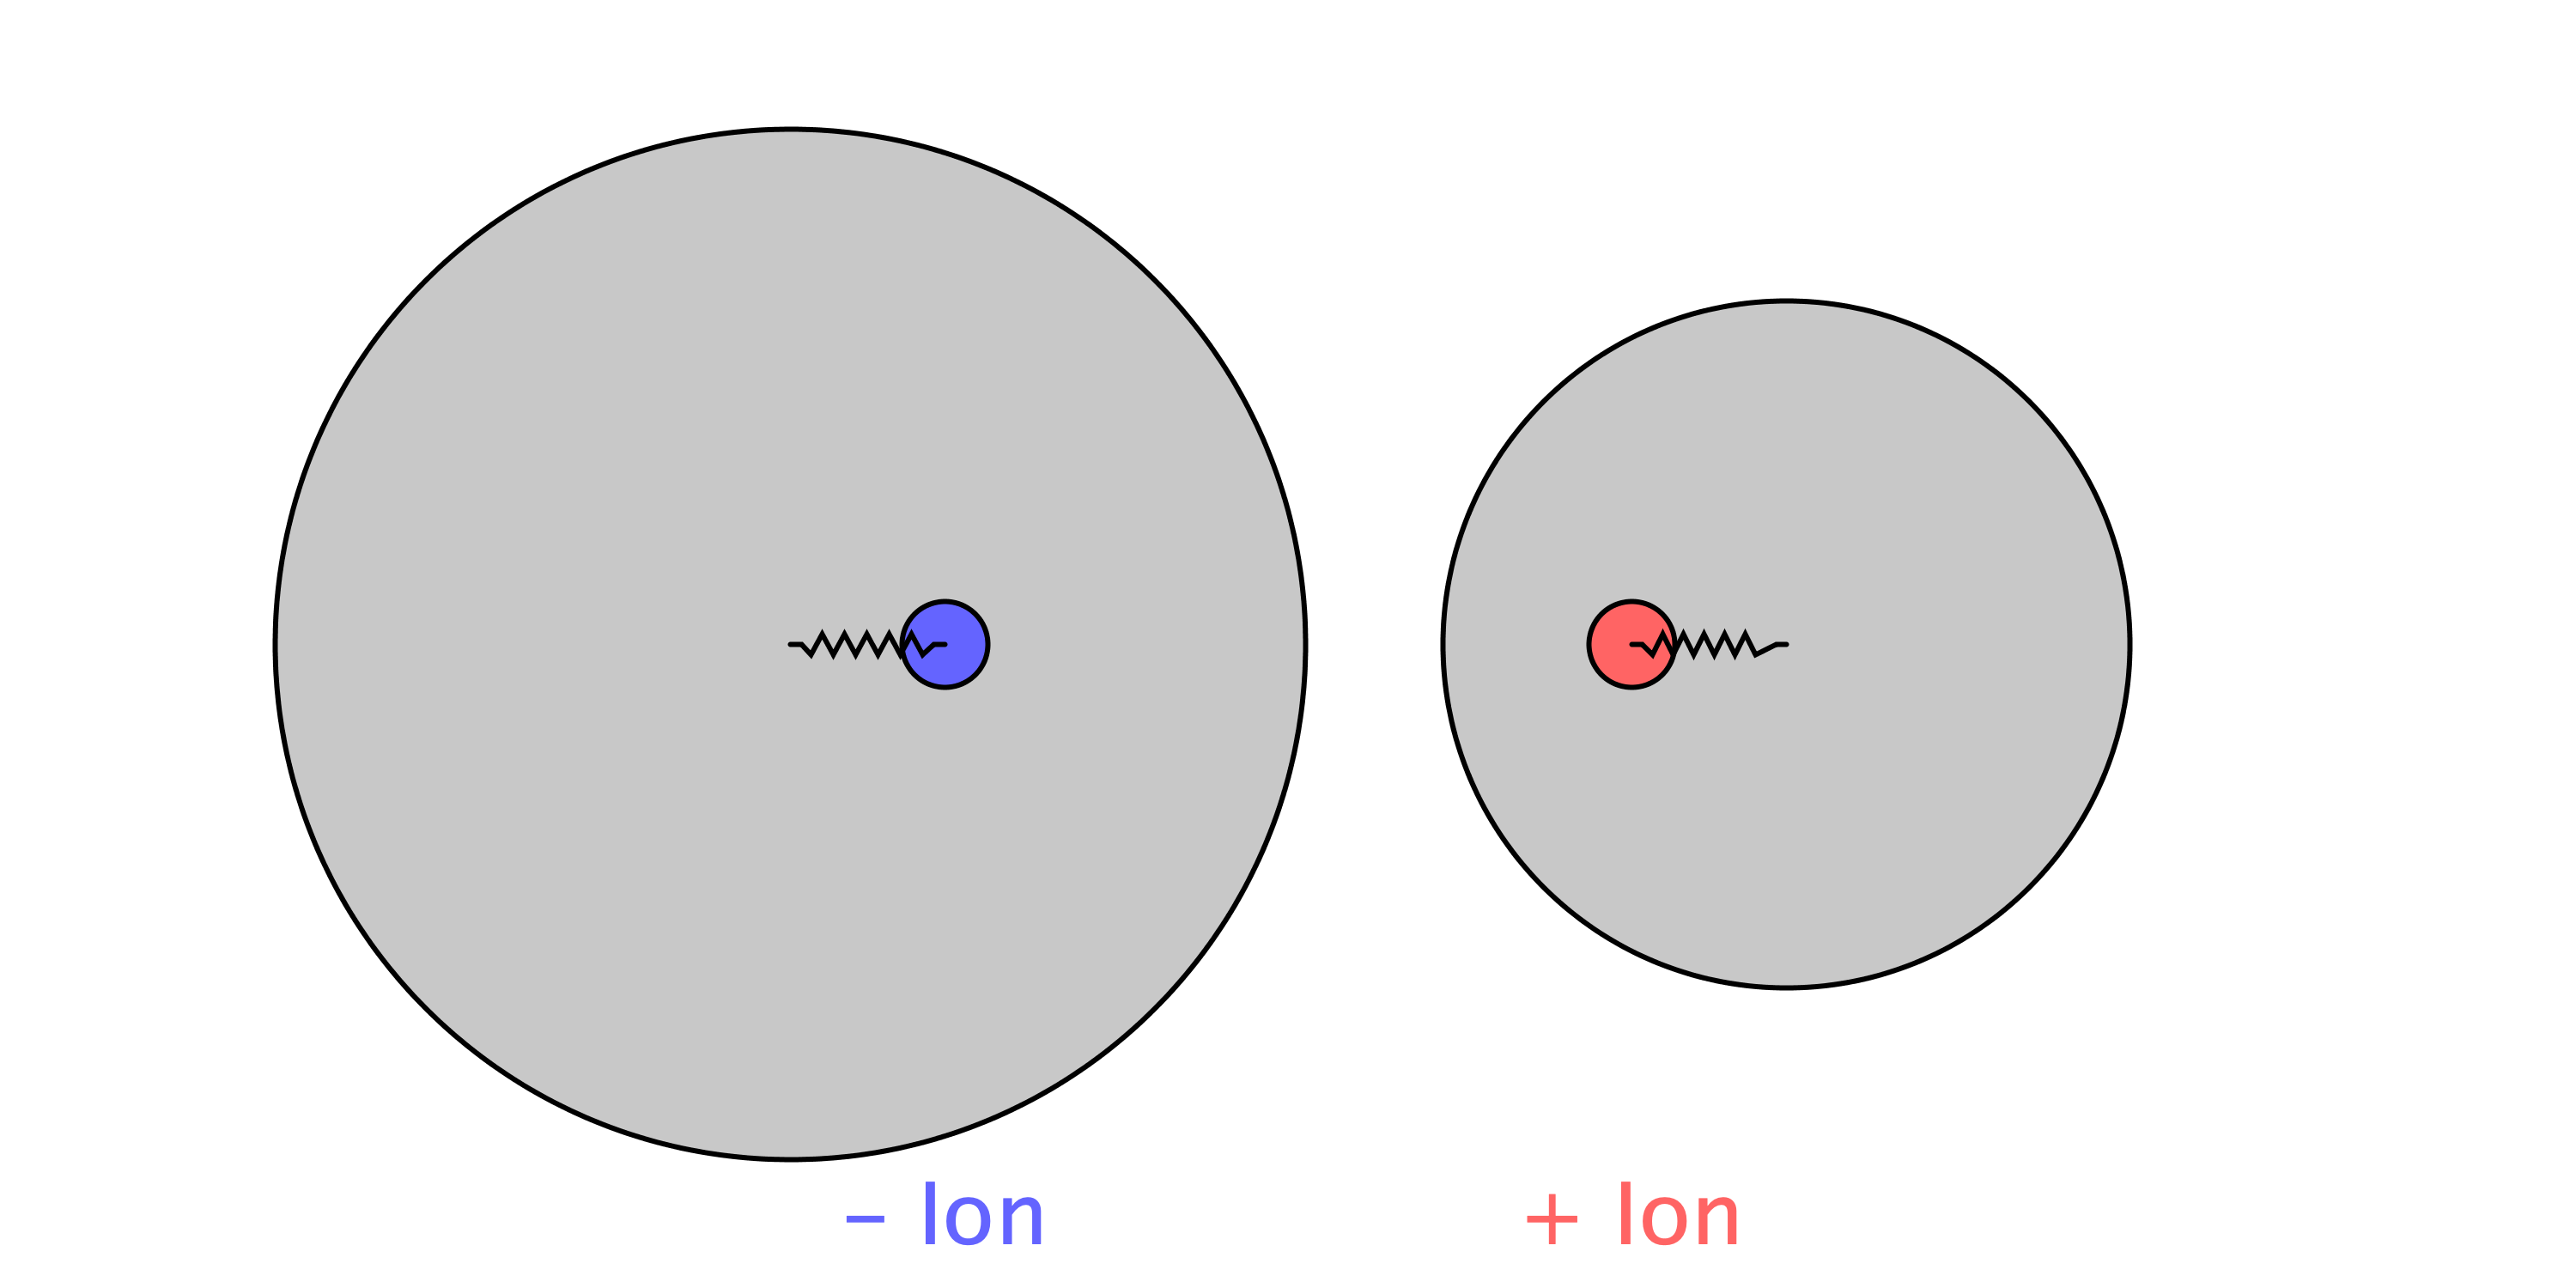
\includegraphics[width=\linewidth]{figures/coreshell/coreshell}
  \caption[Shell model schematic]{Schematic of the shell model of polarisability. The valence electron shells (grey) are attached to the ion core by a harmonic spring, and are displaced by nearby charged species or net electric fields.}
\end{figure}
The shell model\cite{Dick1958} is another computationally inexpensive model of polarisation which accounts for polarisation coupling, thus overcoming a key limitation of the PPI model.
Polarisation coupling is modelled by treating the valence electron cloud as a shell connected to the ionic core by a harmonic spring.
The core represents the nucleus and core electrons of the ion, accounting for the majority of the mass of the ion, while the shell is represents the polarisable valence electrons.
The mass of the shell is treated as zero in non-dynamical systems (i.e. in structural optimisation, Section \ref{sec:minimization}) where the solver strategies are able to handle zero-mass species without instability.
In the case of dynamic systems (i.e. Molecular dynamics, Section \ref{sec:MD}), the shell is assigned a small portion of the overall mass to provide a degree of inertia and remove the need for prohibitively small time-steps.

By allowing the displacement of valence electrons from the ion core, an effective dampening of the polarisation occurs, offering better agreement with experiment.

The charges assigned to the core and shell respectively must sum to that of the point charge it replaces, but the values of these and the spring constant are typically empirically derived.
This polarisation model generally gives good agreement with experiment for ionic halides and oxides.

\section{Partial occupancy and disorder}
Partially occupied sites are those which have no fixed species occupying them, but instead contain vacancies, or some species in a known ratio when summed throughout the whole material.
Disordered solids contain partially occupied lattice sites where the species (or lack thereof) shows no regular ordering in space, instead being randomly distributed throughout the material.



One strategy for addressing this is to use the mean-field approximation. 
At each partially occupied site, the interatomic potentials are calculated as usual for each species which occupies the site. 
The forces are then scaled according to the relative occupancy of each species:

$$
U_{ij} = o_io_jU_{ij}
$$

The sum of these scaled potentials yields the mean potential arising from the partially occupied site.
This technique can be powerful for initial studies of systems in that it yields symmetric (and thus robust) systems, and bypasses the cost issues arising from the combinatorics of generating large systems capturing all likely local environment.
It is particularly useful for the calculation of structural properties, where the averaging of forces is in effect done when determining large scale parameters.

That said, the simplification of lattice sites fails to capture the nuance of local environments, potentially missing properties that might only arise in environments containing certain configurations of species.
As such, caution should be exercised when applying this technique to calculate diffusion barriers.
Furthermore, the implementation of this technique is poorly compatible with the core-shell model in GULP, preventing their simultaneous usage.

Another strategy for handling partially occupied and disordered systems is the supercell approach.
The primitive cell is expanded to be repeated a given number of times in the direction of each basis vector, yielding a supercell.
Each partially occupied site is then assigned one of the species potentially occupying it, such that the desired stoichiometry is achieved across the whole supercell.

Assigning these sites it itself a problem to which many strategies can be applied.
The brute force approach of testing all configurations in not viable for all but the simplest of systems due to the combinatorial nature of the problem.
A simple example of distributing 50 ions and 50 vacancies across 100 symmetry inequivalent sites yields $\frac{100!}{50!\cdot50!} = 10^{29}$ distinct cases.

Another strategy is to randomly assign a species to each site, weighted by stoichiometry.
It is worth clarifying that while perfect disordering is possible, the energetics associated with the formation of a given local environment may bias such systems to exhibit certain local configurations preferentially.
As an example, a disordered rocksalt with a small portion of vacancies at the anionic site might na{\"i}vely be expected, in a sufficiently large system, to have some cationic sites surrounded by six vacancies.
However, the energetics associated with the formation of this local environment would significantly reduce the likelihood of its formation.

Accounting for this when attempting to generate disordered supercells is non-trivial, as the energetics of the environment are not known ahead of time, and the law of large numbers dictates that these sites will form if not biased against.
Further, the potential models used may not be suitable for modelling such unfavourable environments.
Indeed, this problem becomes even more challenging when seeking to derive potentials to fit a disordered system, as the potentials are needed in order to calculate the energetics of the local environments, yielding a {\color{red} chicken and egg type} issue.

A final strategy is to approximate the disordered solid as being ordered.
A benefit of this strategy is it can be coupled with DFT studies to predict low energy ordered structures as a basis for the calculation.
Further, this technique typically yields smaller supercells, making studies in GULP (where periodicity can be leveraged to speed up calculations) significantly cheaper.
Finally, the increased symmetry and reduced number of local environments present makes finding a robust set of potentials easier for such systems.

This of course relies upon a means of generating a low energy or ground state structure for the system being studied, which is itself a non-trivial matter.
One such strategy, cluster expansion, \cite{Bhandari2019} was utilised by the authors of source material for this report, and may be implemented by the author in future work.


\section{Energy minimisation}
\label{sec:minimization}
\subsection{The configuration space}
\label{sec:config}
The internal energy of an ionic system is a function of its atomic coordinates.
While such systems are more easily thought of as a series of points in a 3-space, the resultant energy surface is $3n$ dimensional for a system containing $n$ atoms, with each point on this surface corresponding to a unique set of atomic coordinates.
We define the vector of positions of these atoms, the configuration space, $\mathbf{x}$.

Whilst each position in the configuration space has an associated energy, $U(\mathbf{x})$, real systems tend towards more energetically favourable states.
Stationary points on the energy surface, those where $\nabla U(\mathbf{x}) = 0$, are of particular interest:
\begin{labeling}{\textbf{Saddle point}}
	\item [\textbf{Minima}] Points on the energy surface where:
	\begin{equation}
	\nabla^2 U(\mathbf{x}) > 0
	\end{equation}
	\noindent
	These points correspond to stable structures.
	Multiple minima may exist, corresponding to different configurations or phases that the system can occupy, while the lowest energy minima, the global minima, corresponds to the ground state of the system.
	\item [\textbf{Saddle point}] The point corresponding to the maximum energy whilse taking a minimum energy path between two minima.
	These points correspond to transition states, and are of interest when studying phase changes or ion migration.
\end{labeling}

It is worth noting that whilst it is trivial to confirm that a point is stationary, it is not possible to establish whether a point is globally minumum without an exhaustive search,
Some techniques such as Monte-Carlo methods can, with sufficient run time, identify points which are most likely globally minimum, but for all but the simplest systems, a global search is infeasible.\cite{Barnes1992}


As local minimisation techniques yield the global minimum so long as initialised near the final value, good initial conditions derived from experiment, \textit{ab initio} studies, or an educated guess can obviate the need for global optimisers in some cases.

\subsection{Gradient-based methods}

The internal energy of a system at a given point on the energy surface can be expanded into a Taylor series:
\begin{equation}
\label{eq:taylor}
  U(\mathbf{x}+\delta \mathbf{x}) = U(\mathbf{x}) + \frac{\partial U}{\partial \mathbf{x}} \delta \mathbf{x} + \frac{1}{2!} \frac{\partial ^2 U}{\partial \mathbf{x}^2}(\delta \mathbf{x})^2 \cdots
\end{equation}

Truncating this equation at the second term yields the energy at a given point on the energy surface $U(\mathbf{x})$, and a derivative vector $g$, corresponding to the direction on the energy surface where $U(\mathbf{x})$ increases most rapidly.

\subsubsection{Steepest descent}
In this method, the position in the energy space $\mathbf{x}$ is iteratively updated by:
\begin{equation}
\mathbf{x}_{p+1} = \mathbf{x}_p + g^p\delta
\end{equation}

with an appropriate value of $\delta$ informed by line searches.
The procedure is repeated until some convergence criteria is met.
Whilst calculating the next step is relatively inexpensive, there is no theoretical limit to the number iterations required for convergence.
Furthermore, as for each $\mathbf{x}_p$, $U(\mathbf{x_p})$ must be evaluated, this can be an expensive procedure if evaluating $U(\mathbf{x_p})$ is costly, i.e. for systems with large numbers of species.
This technique also recalculates the gradient vector each step, making no use of information from prior iterations.

\subsubsection{Conjugate gradients}
The conjugate gradients method optimises in $g^0$ on the first iteration, running until a minimum along that vector is found.
$g^1$ is then evaluated and the minimisation procedure is repeated. 
Each new vector is constrained to being orthogonal to all previous search vectors.
If $\mathbf{x}_0$ is sufficiently close to a minima, the energy surface in the search region will be approximately quadratic. 
In this case, the conjugate gradients method converges in $N$ steps for an $N$ dimensional energy surface. 
Put another way, it converges in $3N$ steps for a $N$ body system in 3D space.

\subsubsection{Newton-Raphson Method}
The Newton-Raphson method is a widely used second order minimiser.
Rather than truncating the Taylor expansion of the energy surface (Equation \ref{eq:taylor}) at the first derivative, as in the steepest descent and conjugate gradient methods, an additional second derivative term is included (yielding a Hessian matrix $H$).


\begin{equation}
\Delta \mathbf{x}_p = -H^{-1}g^p
\end{equation}
\begin{equation}
\mathbf{x}_{p+1} = \mathbf{x}_p + \Delta \mathbf{x}_p
\end{equation}

As with the conjugate gradients method, an initial condition near the minima will guarantee convergence, in this case in a single iteration.
That said, outside the quadratic region near minima, the Newton-Raphson method can be numerically unstable.
Furthermore, calculating and inverting the Hessian matrix is a highly expensive.
As such, a BFGS optimiser\cite{Shanno1970} is typically used to update the Hessian between iterations, only explicitly recalculating it only when a criterion indicating the updated Hessian is likely inaccurate is met.
This is considerably cheaper than a Newton-Raphson method on its own.

Where numerical stability is an issue, conjugate gradients or a steepest descent can be used for an initial pass until close to the minima.
The BFGS optimiser can then be used once in a more stable region of the configuration space.

As it is possible to run optimisers until converged to an arbitrary degree of precision (far beyond chemical accuracy), sensible convergence criteria are required to prevent excessively long calculations.
Unless otherwise stated, the default convergence criteria in GULP and LAMMPS are used in this report, with any results presented having converged to at least the degree of precision reported.

\newpage
\section{Periodic boundary conditions}
\begin{figure}[hb]
  \centering
  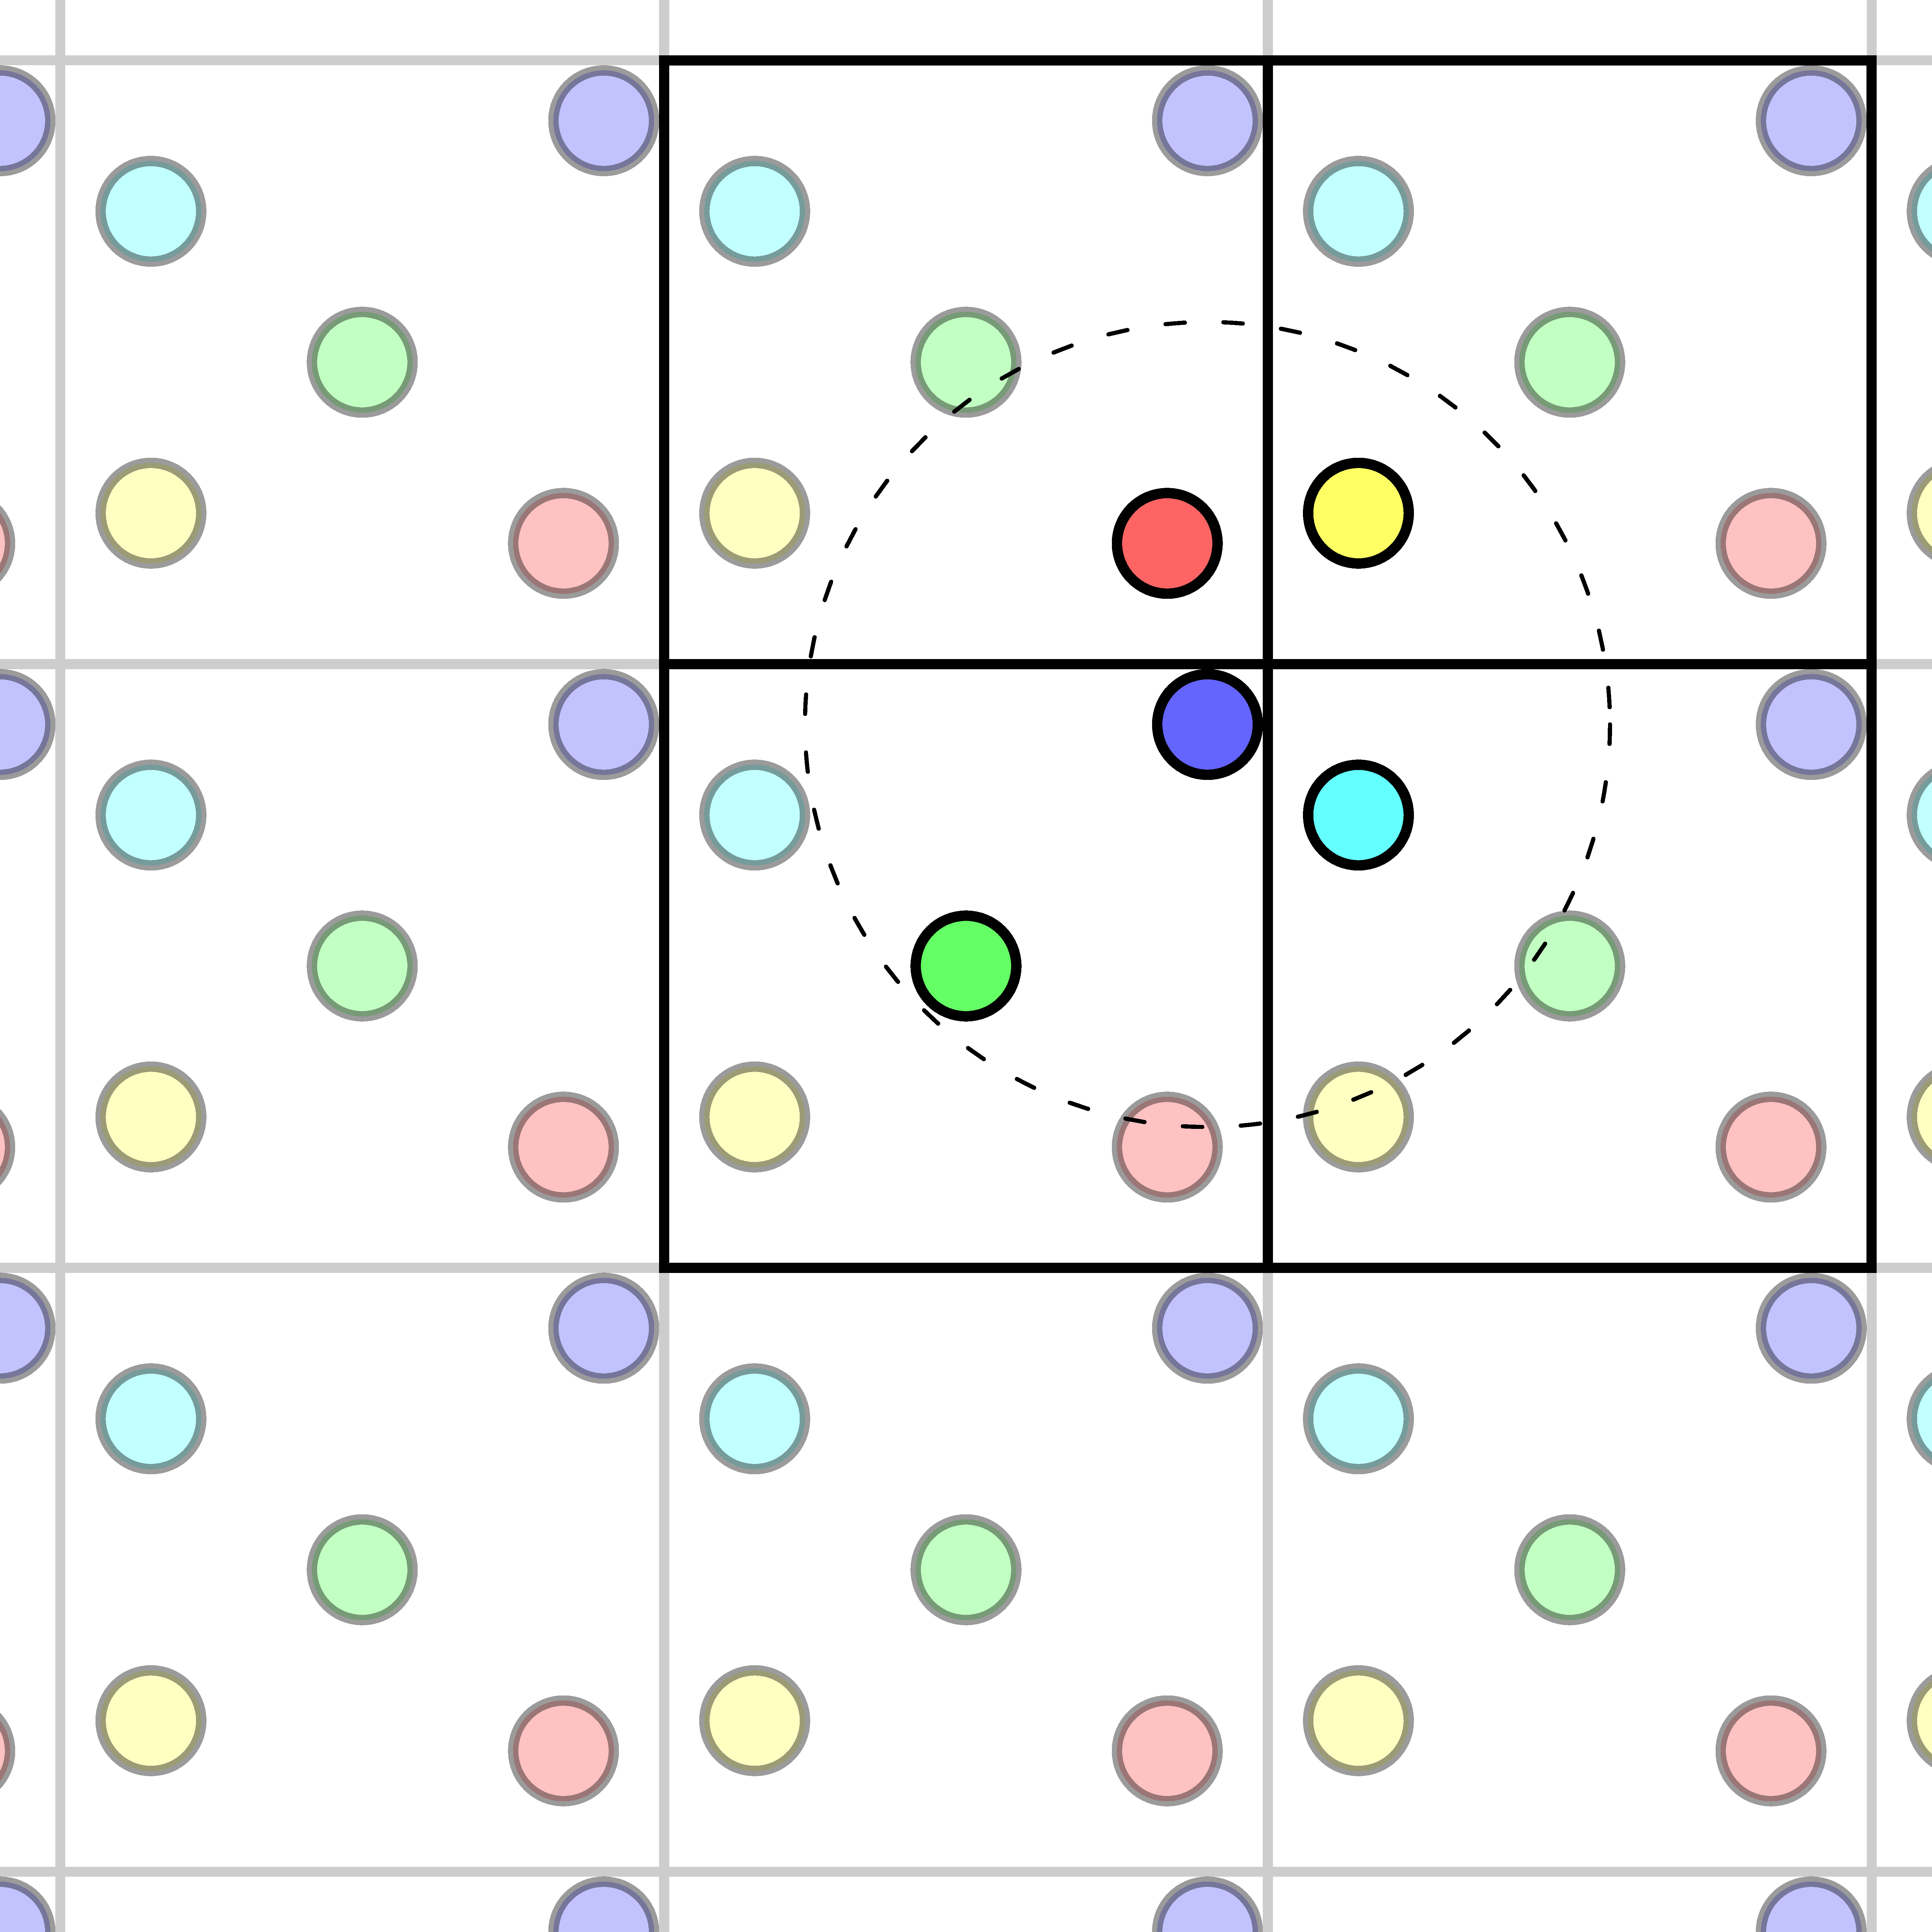
\includegraphics[width = 0.4\linewidth]{figures/pbc/pbc}
  \caption[Periodic boundary conditions schematic]{Schematic of a simulation using periodic boundary conditions.}
  \label{fig:periodic}
\end{figure}
At the scale of atomistic modelling, the materials being studied effectively stretch out infinitely relative to the scale of short-range and Coulombic interactions.
It is of course not feasible to model these systems as such, so boundary conditions which closely approximate this are needed.

Periodic boundary conditions (Figure \ref{fig:periodic}) take the contents of the simulation, and create copies of it at each boundary.
When calculating interactions, species in the ``main'' simulation are able to interact with other species in the main simulation, and those in the repeated simulations, subject to cutoff criteria applied to said interactions.
As the system is infinitely repeating, each copy of an atom must by definition be experiencing the same net force as each of its copies.
As such, it is sufficient to calculate the forces for a single cell only.

Another important of periodic boundary conditions is that atoms which would leave the boundaries of the simulation in the next iteration or time-step are reintroduced at the opposite boundary.
For Molecular Dynamics simulations (Section \ref{sec:MD}), this allows for atoms to move freely rather than being constrained to certain positions in order to keep a constant number of bodies in the simulation.
This is particularly useful when studying diffusion, allowing atoms near simulation boundaries to hop to all adjacent sites.


\newpage


\section{Point defects}
Whilst the atomistic modelling techniques already discussed are applicable in the generic case (as can be demonstrated by their suitability when applied to a P1 symmetry group), they have thus far only been discussed in the context of bulk systems.
In solid-state materials, it is often the presence of defects which gives rise to properties of interest, most likely in concentrations far too low to be studied in a periodic system.
As an example, the energy associated with the formation and migration of \ce{Li+} ions in candidate electrode materials is a key metric of their likely performance.

An overview of defect types, as well as the formalisms used in defining defect formation, is given in the appendix.

\subsection{Mott-Littleton method}
The Mott-Littleton method allows for the modelling of one or more defects at infinite dilution.
The perfect crystal structure is first solved using the techniques listed in Section \ref{sec:minimization}, and the converged result used as an initial condition.
Defects are then introduced the system is once more allowed to relax.
The difference in energy of the systems is directly attributable to the perturbation introduced, and is therefore the energy required to form the defect introduced.
Use of a small periodic system would repeat the defect and be equivalent to simulating the defect at high concentration.

Instead, the system is divided into three concentric spherical regions, as illustrated in Figure \ref{fig:mott}.
As the introduction of a single point defect removes symmetry from the system, a periodic approach is not appropriate, nor is the consideration of an infinite system.

\begin{figure}
  \centering
  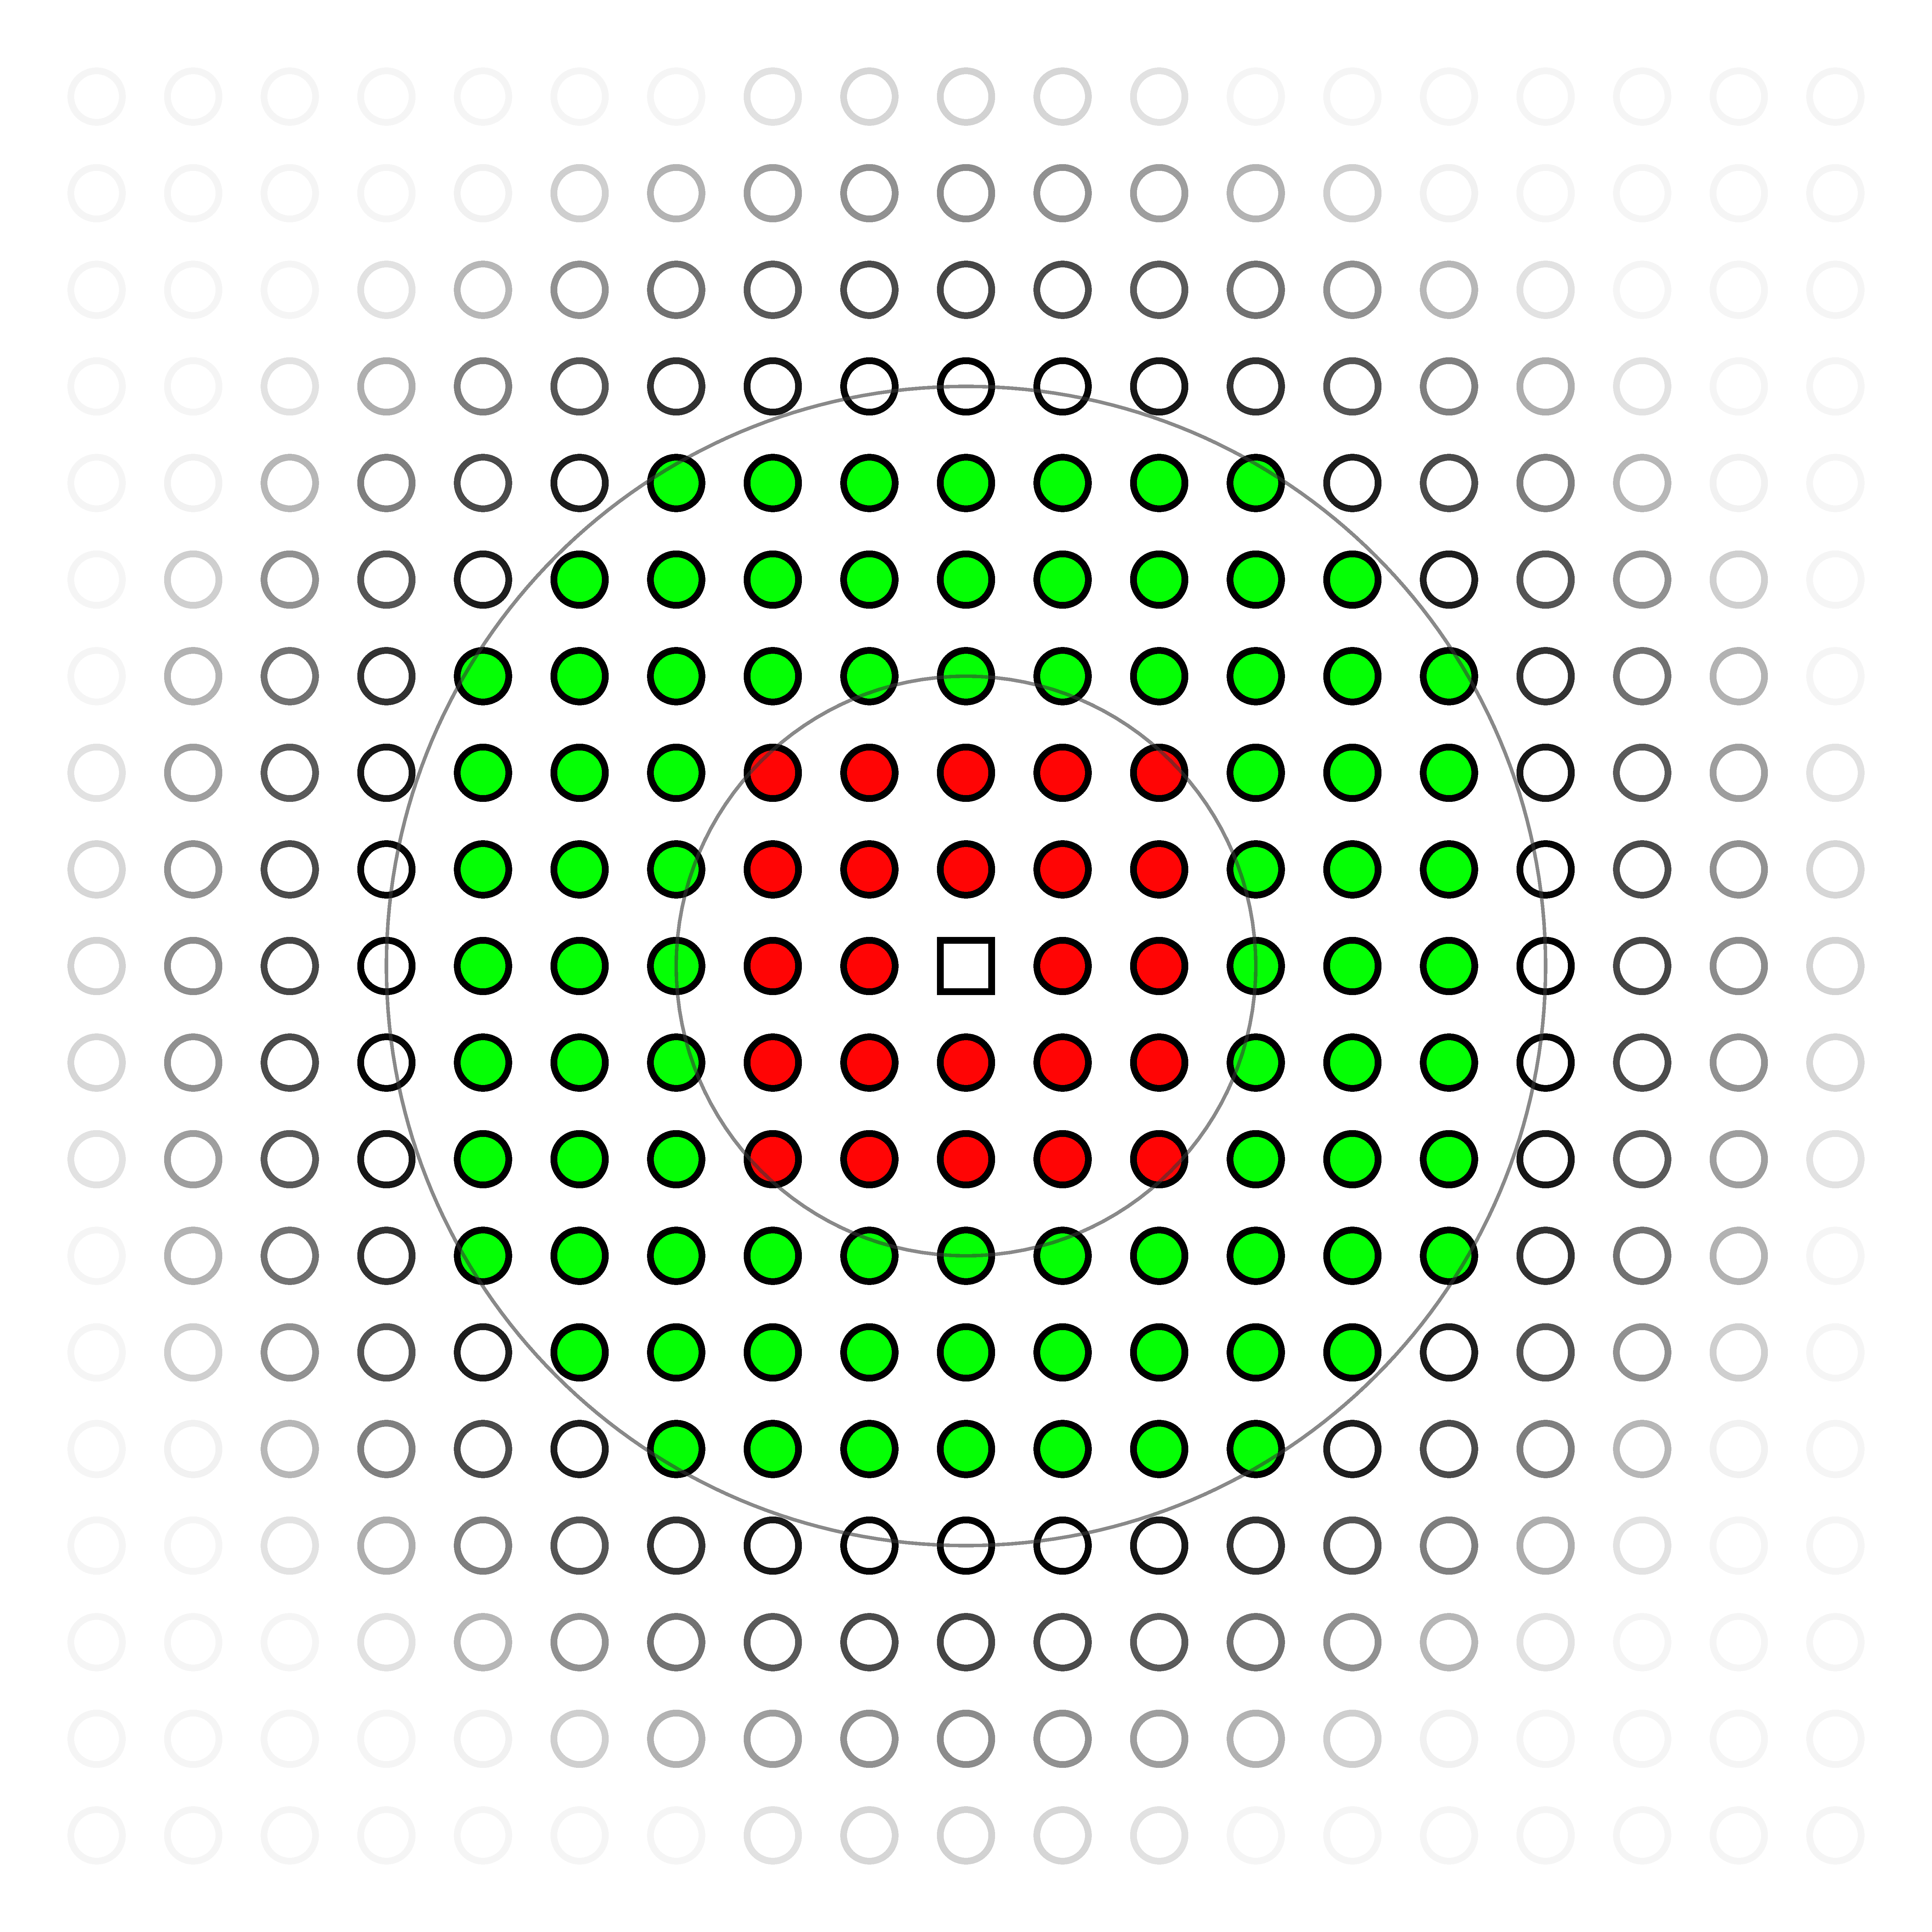
\includegraphics[width = \linewidth]{figures/mott/mott}
  \caption[Mott-Littleton method schematic]{Schematic illustrating the Mott-Littleton method. Ions in region I (green) are modelled explicitly using potential forms due to their proximity to the defect (square). Region IIb ions (white) are modelled using a continuum method. Region IIa ions (green) use a harmonic relationship, smoothing the transition from explicit (Region I) to implicit (Region IIb) modelling.}
  \label{fig:mott}
\end{figure}

Region I contains those ions closest to the defect.
Their close proximity to the defect means no simple approximation can be made to predict the defects impact.
As such, the relaxation of these species is modelled explicitly, using potential models and gradient descent techniques.

Ions in Region II are sufficiently far from the defect to be reasonably approximated using analytical methods.
Region IIb, the outermost region, is sufficiently far from the defect to only impacted by Coulombic interactions with the defect.
These are modelled using a dielectric continuum, the magnitude of the force experienced, and corresponding energy change, being a function of the net charge of the defect and the distance from the defect centre.


Ions in region IIa are modelled as having harmonic interactions with the defect, having an energy cost associated with their displacement from their initial position.
This region smooths the transition between the explicit modelling regime in region I and the implicit modelling regime in region IIb, avoiding discontinuities in the resultant energy surface.

The success of this technique relies upon selection of radii for the regions such that discontinuities do not occur between regions.
Selection of radii intervals greater than the cut-off values imposed on short range interatomic potentials typically achieves this.
That is to say, region IIa should be large enough such that no species in region I have any short range interactions with species in region IIb.

Further, the computational cost of relaxing region I is approximately of {\color{red}$O(r^2!)$}.
As such, a radius for region I should be chosen such that the resultant defect energy does not change with increasing radius, whilst being as small as possible to reduce simulation time.

\subsection{Supercell approach}  
Supercell methods simply take a large supercell of the repeating crystal unit and add a defect to this supercell.
The cell is then modelled as before, with the supercell repeating ``infinitely''.
This approach is limited in that in order to model low defect concentrations, a huge supercell is required.

As such, this method is generally instead only applied in Molecular Dynamics (Section \ref{sec:MD}), where a large concentration of Li vacancies are added in order to allow diffusion events to be observed.

\subsubsection{{\color{red}Symmetry optimisation}} %TODO rewrite
By their nature, crystal structures contain a number of symmetry elements.
In many cases, a number of interactions will be equivalent, enabling the number of computationally expensive operations to be reduced by simply treating some interactions as being equivalent and calculating them once rather than several times.
The addition of defects to a system reduces the overall symmetry of the structure, but there often still exist some symmetry elements.
Symmetry optimised algorithms are automatically implemented where appropriate in GULP.

\section{{\color{red}Molecular dynamics (MD)}}
\label{sec:MD}
Energy minimisation techniques are used to study systems at zero Kelvin.
As such, phenomenon arising only where ions have thermal energy cannot be studied with these techniques.

Molecular dynamics (MD) can overcome this issue by assigning each particle a velocity (usually subject to a Boltzmann distribution) and allows the system to evolve over time subject to some imposed constraints.
This in effect allows for phenomenon arising from thermal effects to be studied,
assigns and tracks kinetic energy of atoms, allowing the system to evolve over time.

The equation which fundamentally governs MD simulations is simply Newtons law of motion:
\begin{equation}
	\mathbf{F} = m\mathbf{a}
\end{equation}

As the force each particle is a function of the positions of each particle in space, which in turn evolves as a function of time, it is necessary to solve this equation repeatedly.

The force acting on each particle is assumed to be constant for some small period of time $\Delta t$.
With this assumption, the position and velocity of each particle at time $t+\Delta t$ can using an Euler integration scheme by:
\newpage
\subsection{Integration schemes}
The Taylor expansion is a technique which allows a function to be expressed as a infinite sum of terms calculated from that functions derivatives at a given point:
\begin{equation}
f(t) = f(t_0 + \Delta t) = \sum_{n=0}^\infty \frac{1}{n!}f^{(n)}(t_0)\Delta t^n
\end{equation}
Applying this to the position of atoms in the system as a function of time yields:
\begin{align}
\mathbf{x}(t_0 + \Delta t) &= &x(t_0) \; &+ &x'(t_0)\Delta t \;&+& &\frac{1}{2}x''(t_0)\Delta t^2 \;&+& \frac{1}{6}x'''(t_0)\Delta t^3& +\;\dots\\
                           &= &x_{t_0} \; &+  &v_{t_0}\Delta t \;&+&   &\frac{1}{2}a_{t_0}\Delta t^2     \;&+& \frac{1}{6}j_{t_0}\Delta t^3& +\;\dots
\end{align}
Truncating this expansion at different terms yields a series of potential equations which can be solved, the discarded terms constituting the error in each step.
The lowest order discarded term will determine the magnitude of the error, with ``simpler'' expansions requiring a correspondingly smaller $\Delta t$ in order to reduce the magnitude of the error to an acceptable value.

\paragraph{Euler integration}
Truncating the Taylor expansion of the position and velocity of particles as a function of time at the first term gives an Euler integration scheme:
\begin{equation}
	\mathbf{v}_{t +\Delta t} = \mathbf{v}_t + \frac{d\mathbf{v}}{dt}\Delta t = \mathbf{v}_t + \mathbf{a}_t\Delta t +\Theta(\Delta t^2)
	\end{equation}
\begin{equation}
	\mathbf{x}_{t +\Delta t} = \mathbf{x}_t + \frac{d\mathbf{x}}{dt}\Delta t = \mathbf{x}_t + \mathbf{v}_t\Delta t +\Theta(\Delta t^2)
\end{equation}
With $\Theta$ representing the error, the brackets indicating the relationship between the size of the error and the choice of time step.
Unfortunately, the $\Theta(\Delta t^2)$ error terms in this integration scheme require a prohibitively small $\Delta t$ to be used for all but the simplest of systems. 

\paragraph{Verlet algorithm} A commonly used integration scheme, the Verlet algorithm, instead truncates the Taylor expansion of the atom positions at the third derivative:
\begin{equation}
\mathbf{x}_{t + \Delta t} = x_{t} \; +  v_{t}\Delta t \;+ \frac{1}{2}a_{t}\Delta t^2     \;+ \frac{1}{6}j_{t}\Delta t^3 + \Theta(\Delta t^4)
\label{eq:verlet1}
\end{equation}
with $j$ indicating the ``jerk'', or rate of change of acceleration of the function.
As the rate of change of acceleration is related to the rate of change of force, the jerk term is not readily calculated.
The Verlet algorithm overcomes this issue by using information known about the system in previous time steps $t_{t}$:
\begin{equation}
\mathbf{x}_{t - \Delta t} = x_{t} \; -  v_{t}\Delta t \;+ \frac{1}{2}a_{t}\Delta t^2     \;+ \frac{1}{6}j_{t}\Delta t^3 + \Theta(\Delta t^4)
\label{eq:verlet2}
\end{equation}

Summing equations \ref{eq:verlet1} and \ref{eq:verlet2} yields:
\begin{align}
\mathbf{x}_{t + \Delta t} + \mathbf{x}_{t - \Delta t} &= 2x_{t} + a_{t}\Delta t^2 + \Theta(\Delta t^4)\\
\mathbf{x}_{t + \Delta t} &= 2x_{t} + a_{t}\Delta t^2 -  \mathbf{x}_{t - \Delta t} + \Theta(\Delta t^4)
\label{eq:verlet}
\end{align}

\noindent allowing for the positions of particles to be calculated at the next time step.
Interestingly, this integration scheme not only obviates determining the rate of change of acceleration of particles, it also skips the calculation of the velocity term.
The Verlet integrator is also time reversible and symplectic (preserves energy), making it suitable for the dynamic systems encountered in MD.
Of course, in order to calculate the kinetic energy of the system, knowledge of particle velocities is needed.
Subtraction of equation \ref{eq:verlet2} from \ref{eq:verlet2} yields:
\begin{equation}
	v_{t} = \frac{x_{t+\Delta t} - x_{t-\Delta t}}{2\Delta t} + \Theta(\Delta t^2)
\end{equation}
giving the Verlet velocity.
As with the $\Theta(\Delta t^2)$ term being too large for calculating the position with a Euler integration scheme, the error term here requires prohibitively small time steps for complex systems.
Velocities are to determine the temperature of the system, which in turn must be a conserved quantity in certain ensembles. %TODO

\paragraph{Velocity Verlet} The Velocity-Verlet algorithm explicitly calculates velocities at half time steps:
\begin{align}
	v_{t +\frac{1}{2}\Delta t} &= \frac{x_{t+\Delta t} - x_t}{\Delta t}\\[10pt]
	&= v_t + \frac{1}{2}a_t\Delta t + \Theta(\Delta t^3)
\end{align}
This half-velocity, the predicted velocity at the time half way between the current and next time step, is then used to update the current positions of ions in the system as in a Euler scheme:
\begin{equation}
	x_{t+\Delta t} = x_t + v_{t +\frac{1}{2}\Delta t}\Delta t + \Theta(\Delta t^4)
\end{equation}

\noindent The velocity at the next time step is then calculated by:
\begin{equation}
	v_{t + \Delta t} = v_{t +\frac{1}{2}\Delta t} + \frac{1}{2}a_{t+\Delta t}\Delta t + \Theta(\Delta t^3)
\end{equation}

Explicitly calculating the velocities in this manner maintains the order of the error in the particle positions, whilst increasing the order of the error in the velocity terms.

It is worth noting that none of the integration schemes are ``self-starting'', that is to say, they are reliant on some initial velocities being known in order to be used.
For a system containing $N$ bodies, velocities will be randomly assigned to give the system a desired initial temperature subject to:
\begin{equation}
	\sum^N_{i=1}m_i\mathbf{v}_i^2 = 3Nk_bT
\end{equation}
whilst ensuring the system has no net momentum in any vector:
\begin{equation}
	\sum^N_{i=1}m_i\mathbf{v} = 0
\end{equation}

One technique currently in development by the author, in collaboration with Dr. Benjamin Morgan and Dr. Lucy Morgan, is to apply a Bayesian approach to potential fitting.
Rather than 
